
\documentclass{subfiles}

\begin{document}
	
\section{Problem and Challenges}\label{sec:Opt:Challenges}
	
	\par While Section \ref{Visualisations} explains a simple approach of extracting a polygonal surface from the voxelised FW LiDAR data, this section is mainly focused on objective No. 5 from table (\ref{tab:Objectives}); it tests the performance of six different data structures on the surface reconstruction and it attempts to improve the interpretation of volumetric data by introducing new data structures. The main challenges raised for this task are because the input data is real laser scanning data that contains noise. Some of the challenges that this chapter attempts to tackle are listed below:
  \begin{enumerate}
		\item The LiDAR sensors are vulnerable to clouds and seagulls being misinterpreted and recorded as hit points. Those outliers are much higher than tree canopies but they are within the boundaries of the scanned area. As a result, on average 97.5\% of the voxels are empty.   	
		\item The Marching Cube, {\color{blue}as described in Section \ref{sec:SurfaceReconstruction}}, is a scan line algorithm, which implies looping through every single voxel, including the empty ones. This is very time consuming and therefore, algorithms that quickly identify and ignore empty areas are essential. 
		\item While loading an entire volume, the huge amount of empty voxels may lead into exceed memory usage. It is therefore preferable to store the voxels into structure that avoids storing the empty ones (i.e. hierarchically).
		\item When extracting a surface from real data, it is very likely to generate non-manifold objects. Non-manifold objects are not homeomorphic to Euclidean 1-space because they have crossing points. This also occurs at the polygonal meshes generated by DASOS as explained at Chapter \ref{Visualisations}.
	\end{enumerate}
	
	{\color{red} ***NEILL: I would make these comments higher level until you have explained more in the chapter. }

	


\section{Related work}
\subsection{Full-Waveform LiDAR Visualisation}

Summarising previous aforemonetioned related work (Section \ref{LiDARsoftwares}), traditional ways of interpreting the full-waveform LiDAR data suggest echo decomposition for detecting peak points and interpreting the point clouds extracted \cite{Wanger2006}. Both SPDlib \cite{Bunting2013} and FullAnalyse \cite{Chauve2009} visualise either the peak extracted points or the raw waveform samples. On the one hand, SPDlib visulises the samples with intensity above a given threshold as points, while FullAnalyse generates a sphere per sample, with its radius directly correlated to the intensity of each wave sample. Similarly, Pulsewaves visualises a number of waveforms with different transparency according to their intensity \cite{Isenburg2012Pulsewaves}. On the one hand, visualising all the wave samples makes understanding of data difficult due to the high noise. On the other hand, peak point extraction identifies significant features but the FW LiDAR data also contains information about echo widths. These information can be accumulated from multiple shots into a voxel array, building up a 3D discrete density volume \cite{Miltiadou2014}. 
\par Voxelisation of FW LiDAR data was introduced by \cite{Persson2005} who used it to visualise small scanned areas (15mx15m). The waveforms samples were inserted into a 3D Voxelised space and the voxels were visualised using different transparencies according to their intensity. Similarly, as explained at Section \ref{Voxelisation}, we adopt voxelisation for surface reconstruction and applied it on larger areas. Once the 3D density volume is generated, numerical implicitisation is used to represent the scanned area. Nevertheless, visualising numerical/implicit objects is not straight forward, since they contain no discrete values (Section \ref{sec:AlgebracObjects}). This problem can either be address by ray-tracing \cite{Hanrahan1983} or polygonisation \cite{Lorensen1987}. In this thesis, the polygonisation direction is taken and a simple approach is explained in Section \ref{sec:SurfaceReconstruction}. This chapter introduces new ways of interpreting real voxelised data and tests how well six data structures and algorithms perform on surface reconstruction.


\subsection{Optimising Volumetric Iso-surface Extraction}
\par Even though volumetric visualisation has only been recently used for FW LiDAR systems, there are many applications in medical visualisation \cite{Levoy1998} \cite{Hadwiger2012} and visual effects \cite{Crassin2009} \cite{Laine2011SparseOctrees}. Research work exists on optimising both ray-tracing and iso-surface extraction (surface reconstruction) and it can be categorised into three groups: surface-tracking, parallelisation and data structures. Those approaches are discussed below along with their benefits and limitations with respect to voxelised FW LiDAR data.

\par Surface-tracking was applied at Rodrigues de Araujo and Pires Jorge \cite{Rodrigues2005} and Hartmann \cite{Hartmann1998}. Starting from a seed point, the surface is expanded according to the local curvature of the implicit object. This method is considered to be faster and more efficient in comparison to the Marching Cubes algorithm since huge empty spaces are ignored. It further opens up possibilities for finer surface reconstruction at areas with high {\color{red}gradient} changes. Nevertheless, surface-tracking algorithms cannot be applied with real laser scanning data because these data are neither manifold nor closed. For example, in a forest scene, a tree canopy may be detached from the ground due to missing information about its trunk. Therefore, by tracking the surface, the algorithm may converged at a single tree instead of the entire forest.  

\par Hansen and Hinker proposed parallelising the polygonisation process of BlobTree trees on Single Instruction, Multiple Data (SIMD) machines \cite{Hansen1992}. {\color{blue}The Instruction is a series of commands to be executed. The longer the series of the commands is, the greater the speed up is. BlobTree trees represent implicit objects as a combination of primitives and operations \cite{Galbraith2004}. As the depth of the tree increases, the length of the parallelised instruction increases as well and therefore a good speed up is achieved}. Nevertheless the function for the implicit representation of the FW LiDAR data at \cite{Miltiadou2014} executes in constant time, making it harder to achieve speed up using SIMD machines. Further, according to the C++ Coding Standards when optimisation is required is better to seek an algorithmic approach first because it is simpler to maintain and less likely to contain bugs \cite{Sutter2004}. 


\par Hierarchical data structures, like octrees, improves the performance of the isosurface extraction because of the huge amount of empty voxels that can be ignored during polygonisation \cite{Wilhelms1990}. The literature in the data structures direction aims to either simplify/improve the output mesh, optimise traversal time of hierarchical data structures or eliminate hierarchy. For example, the extraction of locally finer details either with dual grids \cite{Scott2005} or edge-trees \cite{Wilhelms1992} reduces the amount of vertices produced. In addition, a net of linked surface nodes improved anti-aliasing and reduced artifacts of 3D Magnetic Resonance Imaging {\color{red}(MRI)} \cite{Gibson1998}. Regarding efficiency of accessing data,  franctional cascading slightly improved time complexity of range queries\cite{Chazelle1986}. Sparse Voxel Octrees improved efficiency by having a pointer pointing to children and packing children coherently in memory \cite{Laine2011SparseOctrees}. Hadwiger et al. used a 3D virtual memory to keep voxels coherent on GPU and avoid traversal \cite{Hadwiger2012}. Nevertheless, due to the adjacency of neighbouring voxels, data are saved for empty voxels resulting in much wasted memory. OpenVDB library arranges blocks of grids into a B+ hierarchical data structure for increased cache coherency and lower tree depth \cite{Museth2013OpenVDB}. The bricks stuctured used at GigaVoxels is similar in terms of blocks, named bricks, and it's been used for efficient GPU ray-casting \cite{Crassin2009}. For eliminating tree traversal time, Warren and Salmon introduced hash octrees for N-body simulation of particles \cite{Warren1993hashedOctree}. Similarly, voxel hashing was proposed for reducing the overheads of the traversal time of hierarchical structures and real time surface reconstruction using depth cameras online \cite{Nievner2016voxelHashing}. Most of those data structure optimisations are based on GPU processing, but they are still very relevant.


\section{Overview}



\par This thesis compares six approaches for handling and polygonising voxelised full-waveform LiDAR data. The first three approaches use data structures from the literature and the scan line Marching Cubes algorithm. An explanation of their functionalities is given at Table \ref{tab:DataStructuresScanline}. The last three approaches are more complicated because they take into consideration the chunks of empty voxels and ignore them during surface reconstruction. A brief summary of them is given in Table \ref{tab:DataStructuresOptimised} and an in-depth explanation is given in Sections \ref{sec:IVopt} \ref{sec:OctreeMaxMin} \ref{sec:ITopt} . Please note that the "1D Array" is the original implementation, while each one of the other five approaches tackles at least one of the aforementioned challenges (Section \ref{sec:Opt:Challenges}). 



\begin{table}[!htbp]
	% increase table row spacing, adjust to taste
	\renewcommand{\arraystretch}{1.3}
	% if using array.sty, it might be a good idea to tweak the value of
	% \extrarowheight as needed to properly center the text within the cells
	
	\centering
	% Some packages, such as MDW tools, offer better commands for making tables
	% than the plain LaTeX2e tabular which is used here.
	\begin{tabular}{|P{0.3\textwidth}|P{0.3\textwidth}|P{0.3\textwidth}|}
			
		\hline
		\textbf{1D Array} &	\textbf{Voxel Hashing} & \textbf{Octree}  \\
		\hlinewd{1.5pt}
		Influenced by \cite{Hadwiger2012}, all the data are saved into an 1D array to guarantee coherent memory, even though much memory is wasted in regards of empty voxels. &	The intensities of the voxels are saved into a simple hash table with key value relevant to their position into the volume. Similary to \cite{Nievner2016voxelHashing}, this approach overheads traversing time of hierarchical structures and on top of that it reduces memory allocation because empty voxels are not stored.  &  This is a  hierarchical octree with traversal time to be essential. Please note that this is a scan line test and therefore it does not take into consideration empty chunks of memory.\\	
		\hline
	\end{tabular}
	\caption{Brief Description of the Three Scan-Line Tests}
	\label{tab:DataStructuresScanline}
\end{table}



\begin{table}[!htbp]
	% increase table row spacing, adjust to taste
	\renewcommand{\arraystretch}{1.3}
	% if using array.sty, it might be a good idea to tweak the value of
	% \extrarowheight as needed to properly center the text within the cells
	
	\centering
	% Some packages, such as MDW tools, offer better commands for making tables
	% than the plain LaTeX2e tabular which is used here.
	\begin{tabular}{|P{0.3\textwidth}|P{0.3\textwidth}|P{0.3\textwidth}|}	
		\hline
		\textbf{Integral Volumes} &	\textbf{Octree Max and Min} & \textbf{Integral Tree}  \\
		\hlinewd{1.5pt}
		This data structure is an extension of `Integral Images' to 3D. It was firstly presented at the CGVC conference as part of this thesis. Using Integral Volumes, the sum of any cuboid area is calculated in constant time. By repeatedly dividing the space into cuboids, big empty spaces are quickly identified and ignored during the surface reconstruction. \newline(Section \ref{sec:IVopt}) &	In this approach, the values are saved into an octree, but the surface reconstruction is build along the tree. This is slightly different than a traditional octree, because at each branch node its max and min values are saved. This way, areas that are completely full or empty are identified during traversal before reaching the leaves of the trees. (Section \ref{sec:OctreeMaxMin})  & It is a combination of octree and integral volumes; the sum of a given branch is given at constant time. That was an attempt to combine the idea of `Integral Images' and octrees. Nevertheless, traversal time and backtracking for finding neighbouring voxels still exists. (Section \ref{sec:ITopt})\\	
		\hline
	\end{tabular}
	\caption{Description of the Three Optimisation Attempts}
	\label{tab:DataStructuresOptimised}
\end{table}

\newpage

\section{Integral Volumes}\label{sec:IVopt}
The `Integral Volumes' optimisation is based on the idea of Integral Images, which is an image representation where each pixel value is replaced by the sum of all the pixels that belong to the rectangle defined by the lower left corner of the image and the pixel of interest.  An integral image is constructed in linear time and the sum of every rectangular area is calculated in constant time, as shown in figure \ref{fig:IntegralImages} \cite{Crow1984}


\begin{figure}[!htbp]
	\centering
	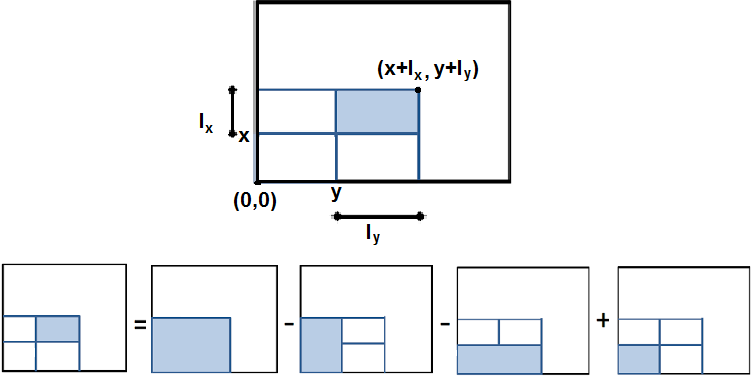
\includegraphics[width=5.5in]{img/IntegralImages}
	% where an .eps filename suffix will be assumed under latex, 
	% and a .pdf suffix will be assumed for pdflatex; or what has been declared
	% via \DeclareGraphicsExtensions.
	\caption[Integral Image]{Once the Integral Image is constructed, the sum of any rectangular area is calculated in constant time.}
	\label{fig:IntegralImages}
\end{figure}


In this thesis, we extend `Integral Images' to `Integral Volumes' and use them to quickly identify aion using depth cameras online \cite{Nievner2016voxelHashing}. Most of those data structure optimisations are based on GPU processing, but they are still very relevant.nd ignore big chunks of empty voxels during polygonisation. The following section explains the mathematics behind `Integral Volumes', while sections \ref{sec:IVoptApproach}  and \ref{sec:IVcodeDetails} give an in depth description about the algorithms invented. 

\subsection{Extending Integral Images to Integral Volumes}\label{sec:extendingIV}

As shown in Figure \ref{fig:IntegralImages},the area of interest is defined by the pixels $(x, y)$ and $(x+l_x, y+l_y)$ and the sum $S$ is given by: 
\begin{equation}
\begin{split}
S = & T(x+l_x,y+l_y) - 
T(x+l_x,y-1)- \\
&  T(x-1,y+l_y) +
T(x-1,y-1)
\end{split}
\label{eq:IntegralImage}
\end{equation}

where 	$S$ is the sum of rectangular area of interest, $T(x, y)$ is the value of the integral image at $(x, y)$ and $l_x, l_y$ define the length of the rectangle in the x and y axis respectively. 

Extending integral images to 3D, the value of the voxel $(x ,y, z)$ in a 3D integral volume becomes equal to the sum of all the values that belong to the box defined by the $(x, y, z)$ and $(0, 0, 0)$ included. 
Therefore the sum $(S)$ of the box defined by $(x, y, z)$ and $(x+l_x, y+l_y, z+l_z)$ included is given by:
\begin{equation}
\begin{split}
S = & T(x-l_x,y+l_y,z+l_z) - 
T(x-1,y+l_y,z+l_z) - \\
&  T(x+l_x,y-1,z+l_z) - 	
T(x+l_x,y+l_y,z-1) + \\
&  T(x-1,y-1,z+l_z)   +
T(x-1,y+l_y,z-1)   +  \\
&  T(x+l_x,y-1,z-1)   -
T(x-1,y-1,z-1)
\end{split}
\end{equation}

where 	$T(x, y, z)$ is the value of the voxel $(x, y, z)$ in the 3D integral volume.  
$S$ is the sum of voxels inside the box, $T(x, y, z)$ is the value of the voxel $(x, y, z)$ in the 3D integral volume. and $l_x, l_y, l_z$ define the length of the box in the $x$, $y$ and $z$ axis respectively. 



\subsection{Optimisation Algorithm}\label{sec:IVoptApproach}
As mentioned before, using `Integral volumes' empty areas are quickly identified and ignored during polygonisation. An iterative algorithm is introduced here. This algorithm continuously splits the volume and checks whether the sub-volumes and its neighbouring voxels are empty using the `Integral Volumes'. Please note that all the values below the threshold boundary of the object must be zero and all the non-empty voxels must contain a positive value.  

\begin{algorithm}
	\caption{Integral Volumes Optimisation Algorithm}
	\label{alg:IVoptSimple}
	\centering
	\begin{algorithmic}[1]
		\State Push the entire Volume as a cuboid inside a Stack
		\While {stack is not empty }
		\State Cuboid-A   $\gets$  next cuboid from the Stack 
		\If{Cuboid-A and neighbours are empty} 
		\State	discard Cuboid-A
		\ElsIf { Cuboid-A consists of only one cube}
		\State polygonise Cuboid-A
		\Else 
		\State divide Cuboid-A
		\State push the two new Cuboids into stack
		\EndIf
		\EndWhile
	\end{algorithmic}
\end{algorithm}
Here it is worth highlighting that, on line 3 of the algorithm it is checked if the neighbouring cubes of a cuboid are empty, because the voxels of the 3D density volume and the cubes in marching cubes algorithm are  aligned with an offset (Figure \ref{fig:ExpectedSampling}). If volumes with non-empty neighbouring voxels are ignored, then holes appear on the output polygon mesh. 		


\begin{figure}[!htbp]
	\centering
	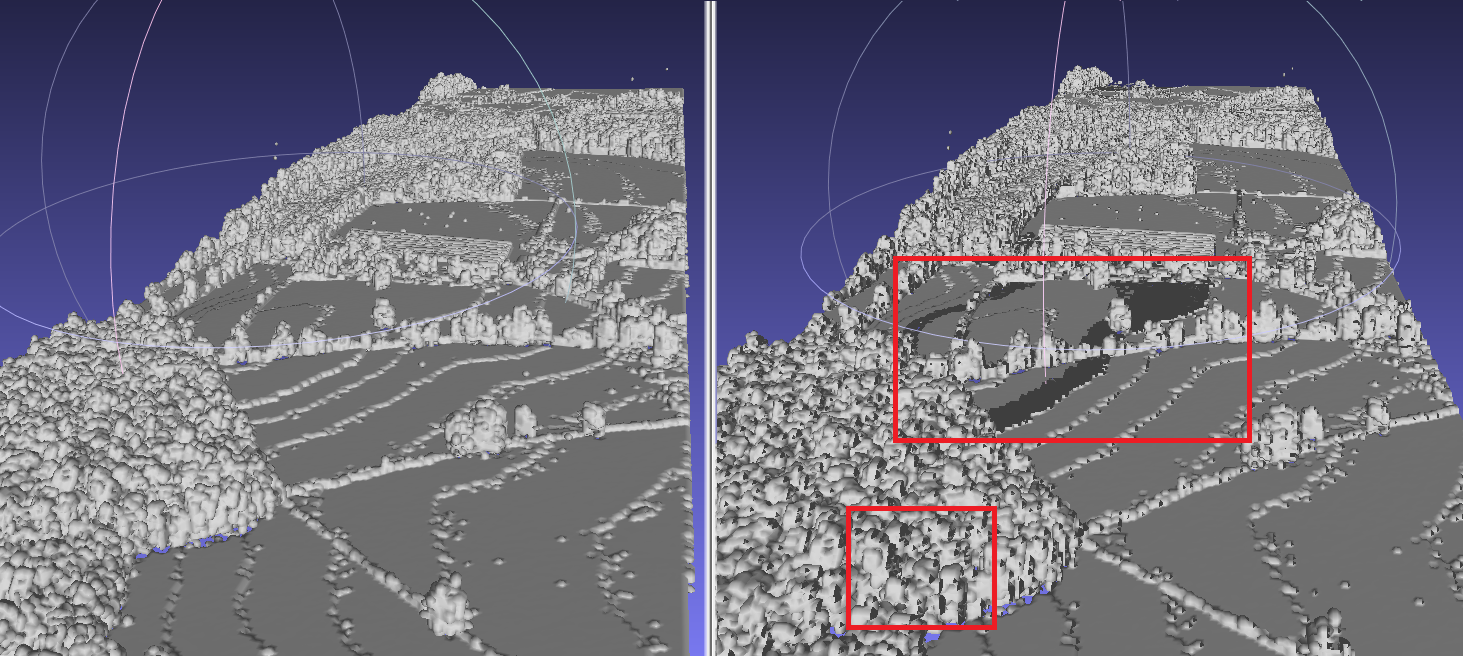
\includegraphics[width=5.5in]{img/HolesNeighbours}
	% where an .eps filename suffix will be assumed under latex, 
	% and a .pdf suffix will be assumed for pdflatex; or what has been eclared
	% via \DeclareGraphicsExtensions.
	\caption{Comparison between including and ignoring neighbouring voxels; holes appears when ignored. {\color{blue} Inside the red boxes, there are two affected areas.}}
	\label{fig:IVholesNeighbours}
\end{figure}

\subsection{Coding Details for Faster Implementation}\label{sec:IVcodeDetails}
Implementation details contributes to the efficiency and speed up of the algorithm. Significant improvements are achieved by reducing recursions, big memory allocations and if statements, since memory jumps are time expensive. As shown in algorithm \ref{alg:IVoptSimple}, a while loop is used to avoid recursion. In this section it's given an explanation on how the stack controls memory consumption and how bitwise operations reduces if-statement usage. 

Regarding memory consumption, a stack was chosen over a queue, to decrease the amount of cubes saved into the data structure simultaneously. A queue is a first in first out data structure, while a stack accesses data in a last in first out order. In every iteration, it is ideal to interpret the smallest saved cube, such that the possibility of being polygonised is higher and the possibility of storing another cube is less. A queue guarantees cubes with approximately the same size, since the big cubes will be added first and sequentially being divided first. In contrast, a stack guarantees the smallest possible number of cubes saved. The larger cubes are stored in the bottom of the stack while the smaller ones are interpreted first because they are always the last one divided and inserted into the stack.  For that reason, a stack guarantees the lowest memory usage. 

Furthermore, in algorithm \ref{alg:IVoptSimple} an issue exists: how to quickly identify the side to be divided next? Ideally, the usage of if-statements should be low because they contains many time expensive memory jumps. For that reason, bitwise operations were embedded into the program to reduce their usage. A cube is defined with its position, its size, the next side to be divided $s$ and its divisible sides $D$. The parameter $s$ takes the values $1$, $2$, $3$ for the $x$, $y$, $z$ sides respectively. The parameter $D$ is an integer consisting of the sum of three numbers $(1$ or $0)+(2$ or $0)+(4$ or $0)$ indicating whether the sides  $x$, $y$, $z$ are divisible or not (table \ref{tab:divisiblesNum}). The parameter $D$ takes the value between $[0,7]$ and covering all the possible cases of divisible sides as shown in tables \ref{tab:Dnumbers} and \ref{tab:Dbinary}. For example if $x$ and $z$ are the divisible sides, then $D = 1+0+4 = 5$. By the end, the bitwise operations and the faster implementations of the Integral Volumes optimisations is shown at algorithm \ref{alg:IVoptAdvance}.



\begin{table}[!htbp]
	% increase table row spacing, adjust to taste
	\renewcommand{\arraystretch}{1.3}
	% if using array.sty, it might be a good idea to tweak the value of
	% \extrarowheight as needed to properly center the text within the cells

	\centering
	% Some packages, such as MDW tools, offer better commands for making tables
	% than the plain LaTeX2e tabular which is used here.
	\begin{tabular}{|P{1.4cm}||P{1.4cm}|P{1.4cm}||P{1.4cm}|P{1.4cm}|}	
		\hline
		&	\multicolumn{2}{c||}{Decimal Numbers} & \multicolumn{2}{c|}{Binary Numbers}  \\
		\hline\hline
		Side &	Divisible & Not\newline Divisible &	Divisible &	Not \newline Divisible  \\
		\hline
		X &	1 &	0 &	0001 &	0000  \\	
		\hline
		Y &	2 &	0 &	0010 &	0000  \\
		\hline
		Z &	4 &	0 &	0100 &	0000 \\
		\hline
	\end{tabular}
	\caption{Values of divisible sides}
	\label{tab:divisiblesNum}
\end{table}



\begin{table}[!htbp]
	% increase table row spacing, adjust to taste
	\renewcommand{\arraystretch}{1.3}
	% if using array.sty, it might be a good idea to tweak the value of
	% \extrarowheight as needed to properly center the text within the cells
	\centering
	% Some packages, such as MDW tools, offer better commands for making tables
	% than the plain LaTeX2e tabular which is used here.
		\begin{tabular}{|P{0.7cm}||P{0.7cm}|P{0.7cm}|P{0.7cm}|P{0.7cm}|P{0.7cm}|P{0.7cm}|P{0.7cm}|P{0.7cm}|}	
		\hline
		X &	1 &	- &	1 &	- &	1 &	- &	1 &	- \\	
		\hline
		Y &	2 &	2 &	- &	- &	2 &	2 &	- &	- \\
		\hline
		Z &	4 &	4 &	4 &	4 &	- &	- &	- &	- \\
		\hline
		D &	7 &	6 &	5 &	4 &	3 &	2 &	1 &	0 \\
		\hline
	\end{tabular}
	\caption{How to calculate the value of D, which represents the divisible sides of a cuboid}
	\label{tab:Dnumbers}
\end{table}


\begin{table}[!htbp]
	% increase table row spacing, adjust to taste
	\renewcommand{\arraystretch}{1.3}
	% if using array.sty, it might be a good idea to tweak the value of
	% \extrarowheight as needed to properly center the text within the cells
	\centering
	% Some packages, such as MDW tools, offer better commands for making tables
	% than the plain LaTeX2e tabular which is used here.
	
	\begin{tabular}{|P{0.7cm}||P{0.7cm}|P{0.7cm}|P{0.7cm}|P{0.7cm}|P{0.7cm}|P{0.7cm}|P{0.7cm}|P{0.7cm}|}
		\hline
		X &	0001 &	-	 &	0001 &	-	 &	0001 &	-	 &	0001 &	-   \\
		\hline
		Y &	0010 &	0010 &	-	 &	-	 &	0010 &	0010 &	-	 &	-   \\
		\hline
		Z &	0100 &	0100 &	0100 &	0100 &	-	 &	-	 &	-	 &	-   \\
		\hline
		D &	0111 &	0110 &	0101 &	0100 &	0011 &	0010 &	0001 &	0000\\
		\hline
	\end{tabular}
	
	\caption{How to calculate the value of divisible sides (D) in binary representation}
	\label{tab:Dbinary}
\end{table}



\begin{algorithm}[!htbp]
	\caption{Integral Volumes Optimisation Algorithm}
	\label{alg:IVoptAdvance}
	\centering
	\begin{algorithmic}[1]
		\State Push the entire Volume as a cuboid inside a Stack
		\While {stack is not empty }
			\State Cuboid-A   $\gets$  next cuboid from the Stack 
			\If{Cuboid-A and neighbours are empty} 
				\State	discard Cuboid-A
			\ElsIf { $D$ is equal to $0$}
				\State polygonise Cuboid-A
			\ElsIf { $( D$ bitwise add $2^s )$ shift right $(s-1)$ }
				\State	divide side s of Cuboid-A 
		
				\If { the new length of side $s$ is equal to $1$ } 
					\State	$D \gets D$ bitwise add $(7-2^s)$
				\EndIf
				\State 	$s \gets (s+1) \text{ mod } 3$
				\State push both new Cuboids into stack
			\Else 
				\State $s \gets (s+1) \text{ mod } 3$
				\State push Cuboid-A back into the stack
			\EndIf
		\EndWhile
	\end{algorithmic}
\end{algorithm}

\newpage

\rhead{ }
\section{Octree Max and Min} \label{sec:OctreeMaxMin}

\par `Integral Volumes' quickly identifies and ignores empty spaces during polygonisation (tackles the 1st, 2nd and 4th problem of the original algorithm -- Section \ref{sec:Opt:Challenges}), but it allocates memory for the entire volume (the 3rd problem). For that reason, the `Octree Max and Min' data structure has been implemented. 

\par The `Octree Max and Min' data structure avoids storing empty voxels and it also identifies empty areas during polygonisation. The polygonisation is built on the traversal of the octree, as explained in Algorithm \ref{alg:MCOctree}. Similarly to `Integral Volumes', a stack is used to avoid recursion and reduce memory jumps. As in the `Integral volumes', it is essential to check neighbouring voxels when a branch of the `Octree Max and Min' data structure could be ignored. However, because the branches of the octree are always a cube, it is not trivial to check whether they are empty or not. For that reason, if a branch is empty then we loop through its edges and polygonise them according to look up table of the the Marching Cubes algorithm. 


\begin{algorithm}[!htbp]
	\caption{Embedding the Marching Cubes Algorithm into an octree structure}
	\label{alg:MCOctree}
	\centering
	\begin{algorithmic}[1]
		\State Push the Root as a Node into a Stack
		\While {stack is not empty }
		\State Node-N   $\gets$  next Node from the Stack 
		\If{ Node-N is a Leaf}
		\State polygonise Leaf
		\ElsIf{Node-N has no children OR max value of Node-N < isolevel \newline OR min value of Node-N > isolevel} 
		\State Polygonise edges of cubic with root node-N	
		\Else
		\State push the children of Node-N into the Stack
		\EndIf
		\EndWhile
	\end{algorithmic}
\end{algorithm}




\par Embedding the polygonisation of volumetric data into an octree has been done before \cite{Wilhelms1990}. Nevertheless, the `Octree Max and Mean' data structure differs in two ways:
\begin{itemize}
	\item The max and min values of each branch are stored into the corresponding node to speed up polygonisation. This enables checking whether the leaves of a branch lie either only inside or only outside the implicit object{\footnote{Explanation about implicit/algebraic objects is given at Section \ref{sec:AlgebracObjects}}}. If they do, then no iso-surface is crossing that branch and it can be discarded (after polygonising its edges).
    \item A new algorithm is proposed and implemented for finding neighbouring voxels. This algorithm reduces comparisons and jumps in memory. An in-depth explanation of this algorithm is given at Section \ref{sec:NeighboursFinding}.
\end{itemize}





\subsection{Finding Neighbours}\label{sec:NeighboursFinding}

\par Every time a voxel/leaf is polygonised, seven of its neighbours are checked to decide whether a surface is passing through that area or not. In hierarchical data structures, the nearest common ancestor is tracked upwards and the branch, with its root as the common ancestor, is traversed to reach the neighbour. The article \cite{Hanan1989} uses recursion that terminates once a common ancestor between a leaf and its neighbour is identified. According to Scharack \cite{Schrack1992}, finding neighbours in linear octrees\footnote{{\color{blue} Linear octrees are octrees whose leaf nodes are stored into a linear array. }} is done in constant time. Nevertheless, linear octrees are full octrees. Therefore, if used in our application, all the empty voxels would have to be stored as well. Lohner suggested vectorising the space during post-processing for finding the shortest distance between un-constructed points \cite{Lohner1994}. However, the 3D voxelised FW LiDAR is a regular grid and, during polygonisation, the shortest distance to travel is one voxel. For that reason, simpler approaches with less initialisation time, like \cite{Schrack1992}, could perform equally well. Castro et al. \cite{Castro2008} assume that with hierarchical octrees it is not possible to find neighbours from leaves and suggest using hashed octrees to do that. In contrast, it is possible to start from the leaves and find the common ancestor using parentship as described at \cite{Hanan1989}.

\par To avoid recursion and reduce comparison, this thesis introduces a new way of finding the  common ancestor using logarithms of $2$. The Algorithm \ref{alg:Ascestor} explains the proposed method. As shown in Figure \ref{fig:OctreeNeighbours}, there are occasions where it is cheaper to start searching a neighbour from the root instead of the leaf. For example Node-$F$ is the $(+1)$ neighbour of Node-$E$. If we start looking for it from the leaves then we need to travel through 6 nodes, but if we start from the root we only need to travel 5 nodes. Logarithms helps us decide which route to take, while reducing comparisons since it is not required to check whether branches has common faces while travelling upwards\cite{Hanan1989}.

\begin{algorithm}[!htbp]
	\caption{Finding the number of upward steps required to reach the common ancestor of a Leaf$(x)$ of interest and its $(+1)$ neighbour}
	\label{alg:Ascestor}
	\centering
	\begin{algorithmic}[1]
		\State $c $  $\gets$ ceil$(log_2 x)$
		\State $c_1 \gets$ ceil$(log_2 (x+1))$
		\While {$c = c_1$}
		\State $x = x - 2^{(c-1)} $
		\State $c $  $\gets$ ceil$(log_2 x)$
		\State $c_1 \gets$ ceil$(log_2 (x+1))$		
		\EndWhile
		\If {$D_{max}/2 < c_1 $}
		\State Start from Root to find Neighbour Branch +1
		\Else
		\State Backtrack $c_1$ parents to find the common ancestor
		\State Find neighbour
		\EndIf
	\end{algorithmic}
\end{algorithm}

\begin{figure}[!htbp]
	\centering
	\includegraphics[width=5.5in]{img/OctreeNeighbours}
	% where an .eps filename suffix will be assumed under latex, 
	% and a .pdf suffix will be assumed for pdflatex; or what has been eclared
	% via \DeclareGraphicsExtensions.
	\caption{This diagram depicts the parameters used for finding neighbouring voxels.}
	\label{fig:OctreeNeighbours}
\end{figure}


\newpage

\section{Integral Tree}\label{sec:ITopt}
\par 

\subsection{Main Idea }

\par The `Integral Tree' is a new term that describes the attempt to preserve some properties of the `Integral Images' while using a non-full tree structure. Every `Integral Tree' consists of two elements: an integral 1D-array and a tree. All the values of every non-empty and non-connecting node are saved into an 1D-array, in a way such that the condition of the `Integral Tree' is fulfilled: all the values of every branch $B$ are adjacent inside the 1D-array. Afterwards the array is converted to integral; the sum of every $n$ continuous values is calculated in constant time. Additionally, the root node of each branch $B$ contains two parameters $(*p, k)$. The number $k$ is the number of nodes, which contain values, of the branch $B$ (e.g. for an octree, it is all its leaf nodes) and the pointer $*p$ points to the first one in the 1D-array (Figure \ref{fig:IntegralTreeMainIdea}).
\par {\color{red} *** NELL:: the *p is a pointer)}

\begin{figure}[!htbp]
	\centering
	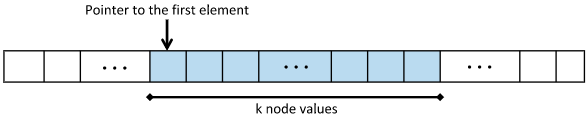
\includegraphics[width=5.5in]{img/IntegralTreeMainIdea}
	% where an .eps filename suffix will be assumed under latex, 
	% and a .pdf suffix will be assumed for pdflatex; or what has been eclared
	% via \DeclareGraphicsExtensions.
	\caption{Ordering of tree elements}
	\label{fig:IntegralTreeMainIdea}
\end{figure}

\par The aforementioned rules can be applied to any tree structures including binary trees, quadtrees and octrees. To better perceive how this data structure works, let’s assume that there is a number of 2D spatially distributed values. Figure  \ref{fig:IntegralTreeQuads} depicts how they can be saved into an `Integral Quad Tree' in order to fulfil the adjacency condition of the `Integral Tree'. Also, Section {\ref{sec:IntegralBinaryTree}} gives an example of an `Integral Binary Tree'.

\begin{figure}[!htbp]
	\centering
	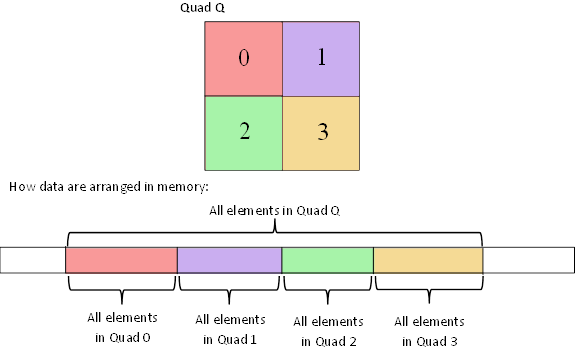
\includegraphics[width=5.4in]{img/IntegralTree}
	% where an .eps filename suffix will be assumed under latex, 
	% and a .pdf suffix will be assumed for pdflatex; or what has been eclared
	% via \DeclareGraphicsExtensions.
	\caption{Illustration of how to save the values of an `Integral Quad Tree' into the 1D-array, in order to preserve the condition of `Integral Trees'}
	\label{fig:IntegralTreeQuads}
\end{figure}


\subsection{Integral Binary Tree Example}\label{sec:IntegralBinaryTree}

\begin{figure}[!htbp]
	\centering
	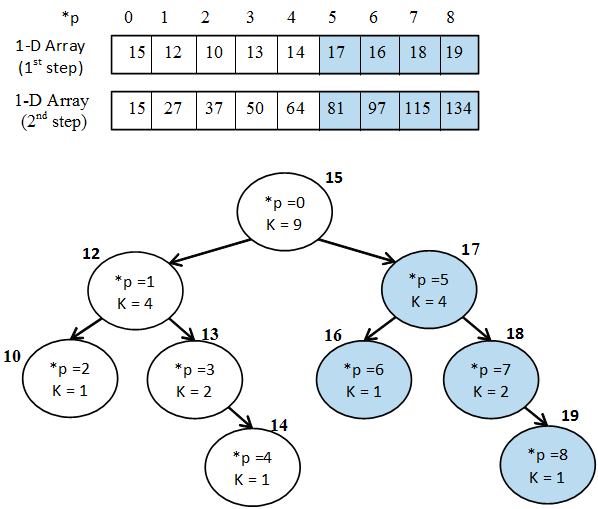
\includegraphics[width=4.8in]{img/IntegralBinaryTree}
	% where an .eps filename suffix will be assumed under latex, 
	% and a .pdf suffix will be assumed for pdflatex; or what has been eclared
	% via \DeclareGraphicsExtensions.
	\caption{Example of `Integral Binary Tree'}
	\label{fig:IntegralBinaryTree}
\end{figure}

\par  An example of applying the idea of `Integral Tree' into a binary tree is given for clarification (Figure \ref{fig:IntegralBinaryTree}). Firstly, the values of the binary tree are sorted into the 1D-array $A$ as $\{15,$ $12,$ $10,$ $13,$ $14,$ $17,$ $16,$ $18,$ $19\}$ in order to fulfil the adjacency condition. Secondly, the array $A$ is modified as $\{15,$ $27,$ $37,$ $50,$ $64,$ $81,$ $97,$ $115,$ $134\}$ in order to become integral using the following equation:
\begin{equation}
\begin{split}
A[i]=A[i]+A[i-1]
\end{split}
\end{equation}


\par Then the sum $S$ of a branch, with ($*p$, $k$) parameters,  is calculated at constant time as follow:
\begin{equation}
\begin{split}
S = A[*p+k-1]-A[*p-1]
\end{split}
\end{equation}

\par For instance the sum of the blue branch on Figure \ref{fig:IntegralBinaryTree} is $A[5+4-1]-A[5-1] = A[8]-A[4] = 134-64 = 70$, which is correct since $17+16+18+19=70$.




\subsection{Integral Octree for Surface Reconstruction}

\par For an `Integral Octree', all the values saved into the integral 1D-array are the values of the leaf nodes since the rest are connecting nodes. For the surface reconstruction, an `Integral Octree' is implemented and the same polygonisation algorithm as `Octree Max and Min' are used (Algorithm \ref{alg:MCOctree} and Algorithm \ref{alg:Ascestor}). The only difference is the comparison at Line 6 of Algorithm \ref{alg:MCOctree}; instead of checking the max and min values, the sum of the branch is checked instead. If the sum is smaller than the iso-surface value then no surface is crossing that area and the branch is discarded. 



\section{Data Structures Summary}

\par To briefly sum up, the following six data structures has been implemented their performance has been tested for reconstructing polygonal meshes from voxelised FW LiDAR data:

\begin{enumerate}
	\item \textbf{1D-Array}: Simple array that keeps data coherent in memory for quick access.
	\item \textbf{Voxel Hashing}: A hashed table is used for storing the intensity values of the voxels \cite{Nievner2016voxelHashing}.
	\item \textbf{Octree}: Simple hierarchical structure with a scan-line implementation.
	\item \textbf{Integral Volumes}: Extension of `Integral Images' that allows finding the sum of any cuboid area in constant time. It is a new algorithm and it is used for quickly identifying and ignoring empty areas during polygonisation.
	\item \textbf{Octree Max/Min}: The polygonisation is embedded into an hierarchical data structure \cite{Wilhelms1990}. The max and min values of each branch are stored to identify and ignore branches that either only contain low level noise or are completely inside the implicit object. Logarithms are further introduced for faster neighbouring finding. 
	\item \textbf{Integral Octree}: An attempt to preserve properties from both `Octree Max/Min' and `Integral Volumes'. 
\end{enumerate}

\par Each one of the aforementioned data structure has different properties and attempts to address at least one of the problems mentioned in Section \ref{sec:Opt:Challenges}. The first three implementations are scanline algorithms, which means that polygonisation is linear and all the voxels, including the empty ones, are checked for generating triangles primitives. Some data structures are taken from the literature to test how well they perform on this specific datasets while others are new and presented into this thesis. Table \ref{tab:DataStructuresProperties} summarises their properties and the problems each data structure attempts to resolve. 

{\color{red} ***Neill: Include citations in table for existing scanline algorithms from literature}


\begin{table}[!htbp]
			\small
	% increase table row spacing, adjust to taste
	\renewcommand{\arraystretch}{1.3}
	% if using array.sty, it might be a good idea to tweak the value of
	% \extrarowheight as needed to properly center the text within the cells
	\centering
	% Some packages, such as MDW tools, offer better commands for making tables
	% than the plain LaTeX2e tabular which is used here.
	
	\begin{tabular}{|P{1.3cm}||P{1.75cm}|P{1.9cm}|P{1.5cm}|P{1.5cm}|P{1.8cm}|P{1.7cm}|}

		\hline
   		 &	Scan-line algorithm: loops through all voxels \newline(1)& Identifies and ignores empty areas during polygonisation	(2) &	Avoids storing empty voxels in memory (3)& Works on non-manifold objects \newline\newline(4)& Requires Cubic Boundaries of the voxelised data& New data structure, introduced for this thesis\\
	    \hlinewd{1.5pt}
		1D-Array & \Checkmark	 &	-	 &	-& \Checkmark&-& - \\
		\hline
		Voxel Hashing &	\Checkmark &	- &	-	&\Checkmark&-& - \\
		\hline
		Octree &	\Checkmark &	- &\Checkmark&\Checkmark&\Checkmark& - \\
		\hline
		Integral Volumes &	- & \Checkmark	& - &\Checkmark&-& \Checkmark \\
		\hline
		Octree Max/Min &	- &	\Checkmark&\Checkmark &\Checkmark&\Checkmark& \Checkmark\footnotemark\\
		\hline
		Integral Octree & -	 &	\Checkmark&\Checkmark&\Checkmark&\Checkmark& \Checkmark \\
		\hline
	\end{tabular}
	
	\caption{Summarising the addressed challenges and the properties of all the data structures implemented.The numbers of the first four columns correspond to the challenges described in Section \ref{sec:Opt:Challenges}}
	\label{tab:DataStructuresProperties}
\end{table}

\footnotetext{Integrating polygonisation into an octree has been done before, but there only a few modifications to a normal octree; the max and min values stored into the branch and the introduction of logarithms for finding neighouring voxels.} 

\section{Results and Experiments}

\par The implemented algorithms are beneficial in different aspects: speeding up execution or decreasing memory usage. The performance has been tested within two groups of test cases:

\begin{itemize}
	\item The results of the first group are given in Table \ref{tab:ResultsOptimisationSingleFlightline} and visualised in the Charts depicted in Figures \ref{fig:ConTime}, \ref{fig:PolTime}, \ref{fig:TotalTime} and \ref{fig:MemoryConsumption}
	\item The results of the second group are given in Table \ref{tab:ResultsOptimisationMultiFlightline}. The related charts are inside Table \ref{tab:OptTestGrapshs}. 
\end{itemize}
 \par This section clarifies the various parameters of testing, while the following Section \ref{sec:Opt:Discussion} discussed the results and explains the behaviour of the algorithms in respect to the results. 

\par The two test cases have only one difference, with the rest of the parameters being held the same. The difference is that the first one uses one flightline (the LDR-FW-FW10\_01-201009821.LAS from New Forest) and focuses on its performance using a finer resolution range. In contrast, the second uses three filghtlines from the NERC-ARF datasets. The first flightline is from the New Forest (LDR-FW-FW10\_01-201009822.LAS), the second flightline is from the Dennys Wood  (LDR-FW10\_01-201018713.LAS) and the third one from Eaves Wood (LDR-FW-GB12\_04-2014-083-13.LAS). The second group checks whether there are significant performance differences when the algorithms are applied on different flightlines. 

\par Except for the flightlines used, the rest of the parameters are the same in both test cases. In order to understand the size of the data, the voxel length, the number of voxels in the x,y,z axes and the percentage of empty voxels are stated. The smaller the voxel length is, the more voxels exist because the boundaries of the voxels in meters are constant and when the voxel length decreases the resolution of the volume increases. Additionally, for every resolution, the execution time and maximum memory consumption are measured. Execution time is further divided into data structure construction (including reading the LAS file) and polygonisation. 



{\color{red} *** Neill::: Consider adding log(execution time) in diagrams and sum of voxels per test in the results}




{
\begin{sidewaystable}[!htbp]
	\small
	% increase table row spacing, adjust to taste
	\renewcommand{\arraystretch}{1.3}
	% if using array.sty, it might be a good idea to tweak the value of
	% \extrarowheight as needed to properly center the text within the cells
	\centering
	% Some packages, such as MDW tools, offer better commands for making tables
	% than the plain LaTeX2e tabular which is used here.
	\begin{tabular}{|P{0.9cm}|P{2cm}|P{0.9cm}||P{0.82cm}|P{0.8cm}|P{0.8cm}|P{0.7cm}||P{0.7cm}|P{0.8cm}|P{0.8cm}|P{0.6cm}||P{0.7cm}|P{0.8cm}|P{0.8cm}|P{0.6cm}|}	
    \hlinewd{1.5pt}
		\multicolumn{3}{|c||}{} & \multicolumn{4}{c||}{\textbf{1D-Array}} & \multicolumn{4}{c||}{\textbf{Voxels Hashing}} &\multicolumn{4}{c|}{\textbf{Octree}}  \\
		\hline
		
		\multicolumn{3}{|c||}{Specifications} & \multicolumn{3}{c|}{Time (s)} & \multicolumn{1}{c||} {Memory} & \multicolumn{3}{c|}{Time (s)}&  \multicolumn{1}{c||}{Memory}&\multicolumn{3}{c|}{Time (s)}& \multicolumn{1}{c|}{Memory}  \\
		\hline
		Length (m) & No. of Voxels & Empty& Con & Pol & Total& MByte &  Con & Pol & Total & MByte &  Con & Pol &Total & MByte \\
		\hlinewd{2pt}
		20&	29x115x23& 	93.20\%&	12.04&	0.16&	12.21&	10.17&	12.84&	0.19&	13.02&	9.78&	14.58&	0.18&	14.76&	11.07\\
		15&	39x157x30 &	94.32\%&	12.06&	0.32&	12.38&	12.50&	12.96&	0.37&	13.33&	11.44&	14.91&	0.35&	15.26&	12.00\\
		10&	 58x235x45 &95.08\%&	12.07&	0.8	&	12.87&	20.09&	12.95&	0.96&	13.92&	16.19&	14.92&	0.91&	15.82&	16.69\\
		5&	116x476x89 & 96.38\%&	12.08&	4.85&	16.92&	88.35&	13.01&	6.95&	19.96&	47.66&	15.26&	5.55&	20.81&	50.50\\
		4&	 145x597x111 &	96.81\%&12.24&	9.21&	21.45&	158.94&	13.08&	12.83&	25.91&	76.70&	15.58&	10.61&	26.19&	80.31\\
		3&	 194x800x148& 97.42\%&	12.19&	21.9&	34.09&	362.23&	13.23&	29.94&	43.16&	153.27&	15.67&	24.14&	39.81&	178.27\\
		2&	290x1199x222&98.21\%&	12.45&	67.65&	80.10&	1153.13&13.69&	95.85&	109.54&	389.34&	16.16&	75.29&	91.45&	417.98\\
		1.5&387x1602x295&98.70\%&	12.83&	151.48&	164.31&	2666.67&13.96&	216.35&	230.31&	788.00&	16.26&	166.23&	182.49&	839.35\\
		1&	80x2405x443 &99.24\%&	14.62&	443.5&	458.1&	8556.78&15.43&	672.07&	687.5&	1912.57&16.91&	491.88&	508.79&	2056.805\\

		\hlinewd{1.5pt}
		\hlinewd{2pt}
		\multicolumn{3}{|c||}{} & \multicolumn{4}{c||}{\textbf{Integral Volumes}}  &\multicolumn{4}{c||}{\textbf{Octree Max/Min}}& \multicolumn{4}{c|}{\textbf{Integral Octree}}  \\
		\hline
		\multicolumn{3}{|c||}{Specifications} & \multicolumn{3}{c|}{Time (s)} & \multicolumn{1}{c||} {Memory} & \multicolumn{3}{c|}{Time (s)}&  \multicolumn{1}{c||}{Memory}&\multicolumn{3}{c|}{Time (s)}& \multicolumn{1}{c|}{Memory}  \\
		\hline
		Length (m) & No. of Voxels & Empty& Con & Pol & Total& MByte &  Con & Pol & Total & MByte &  Con & Pol &Total & MByte \\
		\hlinewd{2pt}	
		20&	29x115x23 	&93.20\%	&12.9&	0.15&	13.05&	10.38&	14.65&	0.21&	14.86&	18.32&	15.67&	0.23&	15.9&	18.27\\
		15&	39x157x30 &	94.32\%		&12.11&	0.28&	12.39&	12.80&	16.01&	0.34&	16.35&	19.80&	15.76&	0.37&	16.13&	20.16\\
		10&	 58x235x45 & 95.08\%	&12.17&	0.68&	12.85&	20.43&	16.12&	0.89&	17.01&	25.68&	16.32&	0.92&	17.24&	25.93\\
		5&	116x476x89 &96.38\%		&13.62&	3.56&	16.02&	88.84&	16.31&	4.99&	21.3&	67.50&	16.98&	5.03&	22.01&	68.94\\
		4&	 145x597x111 &96.81\%	&13.32&	6.48&	19.81&	159.08&	16.62&	9.45&	26.07&	110.24&	17.45&	9.67&	27.12&	117.25\\
		3&	 194x800x148& 97.42\%	&15.15&	14.37&	29.52&	363.95&	16.74&	26.16&	42.9&	218.92&	17.51&	26.35&	43.86&	231.67\\
		2&	290x1199x222 &98.21\%	&23.11&	40.80&	63.91&	1154.02&17.21&	63.02&	80.23&	595.01&	18.14&	64.08&	82.22&	720.01\\
		1.5&387x1602x295&98.70\% 	&39.64&	86.54&	126.18&	2667.67&18.37&	131.21&	149.58&	898.8&	21.22&	133.46&	154.68&	1068.43\\
		1&	80x2405x443& 99.24\%	&111.38&210.94&	322.32&	8559.66&19.91&	348.97&	368.88&	2087.71&25.83&	352.31&	378.14&	2223.14\\
	
		\hlinewd{1.5pt}
		
	\end{tabular}
		\caption{Results: Execution time and memory consumption, Con=Construction, Pol= Polygonisation, MByte=Max Memory}
		\label{tab:ResultsOptimisationSingleFlightline}
\end{sidewaystable}

}

\newpage

\begin{figure}[!htbp]
	\centering
	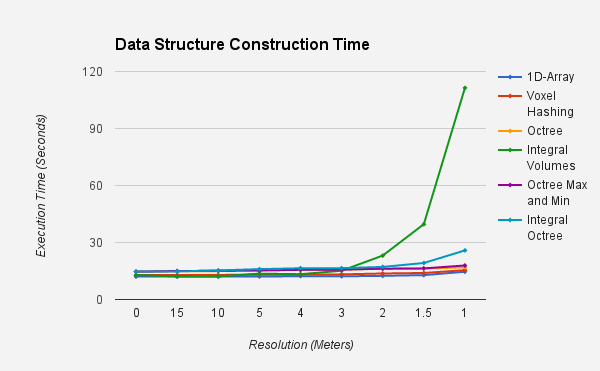
\includegraphics[width=0.8\textwidth]{img/opt/ConstructionTime}
	% where an .eps filename suffix will be assumed under latex, 
	% and a .pdf suffix will be assumed for pdflatex; or what has been eclared
	% via \DeclareGraphicsExtensions.
	\caption{Time required to build each data structure by voxelising the FW LiDAR samples and inserting them inside the 3D volume (Table \ref{tab:ResultsOptimisationSingleFlightline}). Please note that the y-axis is in logarithmic scale.}
	\label{fig:ConTime}
\end{figure}

\begin{figure}[!htbp]
	\centering
	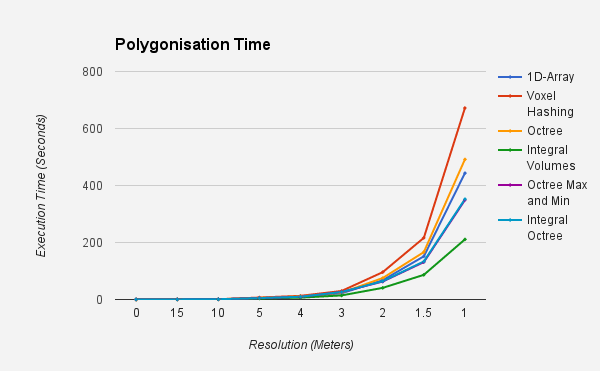
\includegraphics[width=0.8\textwidth]{img/opt/PolygonisationTime}
	% where an .eps filename suffix will be assumed under latex, 
	% and a .pdf suffix will be assumed for pdflatex; or what has been eclared
	% via \DeclareGraphicsExtensions.
	\caption{Time required to reconstruct the surface from the voxelised FW LiDAR data, after the data are voxelised (Table \ref{tab:ResultsOptimisationSingleFlightline}). Please note that the y-axis is in logarithmic scale.}
	\label{fig:PolTime}
\end{figure}

\begin{figure}[!htbp]
	\centering
	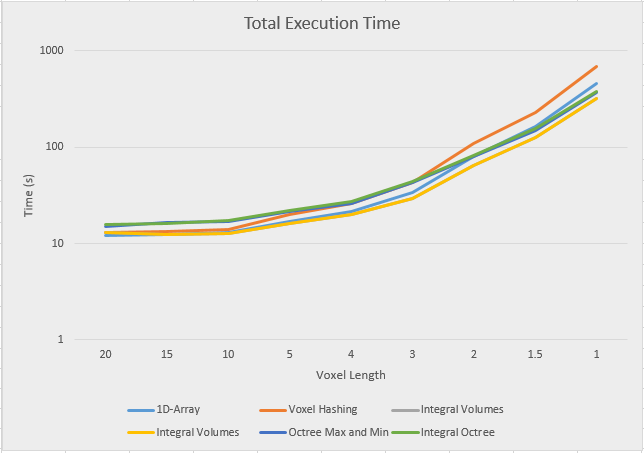
\includegraphics[width=0.8\textwidth]{img/opt/TotalExecutionTime.png}
	% where an .eps filename suffix will be assumed under latex, 
	% and a .pdf suffix will be assumed for pdflatex; or what has been eclared
	% via \DeclareGraphicsExtensions.
	\caption[Total Execution Time]{The sum of the time required to construct a data structure and the time required to generate a polygonal mesh (Table \ref{tab:ResultsOptimisationSingleFlightline}). The fastest one is the `Integral Volumes'. Please note that the y-axis is in logarithmic scale.}
	\label{fig:TotalTime}
\end{figure}

\begin{figure}[!htbp]
	\centering
	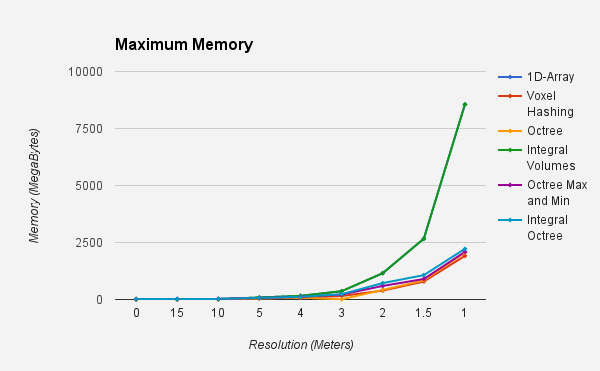
\includegraphics[width=0.8\textwidth]{img/opt/MemoryConsumption}
	% where an .eps filename suffix will be assumed under latex, 
	% and a .pdf suffix will be assumed for pdflatex; or what has been eclared
	% via \DeclareGraphicsExtensions.
	\caption[Maximum Memory Consumption] {Maximum memory consumption at run time. `1D-Array' and `Integral Volumes' consume the highest memory, which is approximately the same (Table \ref{tab:ResultsOptimisationSingleFlightline}). Please note that the y-axis is in logarithmic scale.}
	\label{fig:MemoryConsumption}
\end{figure}


\begin{sidewaystable}[!htbp]
	\small
	% increase table row spacing, adjust to taste
	\renewcommand{\arraystretch}{1.3}
	% if using array.sty, it might be a good idea to tweak the value of
	% \extrarowheight as needed to properly center the text within the cells
	
	\centering
	% Some packages, such as MDW tools, offer better commands for making tables
	% than the plain LaTeX2e tabular which is used here.
		\begin{tabular}{|P{0.9cm}|P{2cm}|P{0.9cm}||P{0.82cm}|P{0.8cm}|P{0.81cm}|P{0.7cm}||P{0.7cm}|P{0.81cm}|P{0.82cm}|P{0.6cm}||P{0.7cm}|P{0.8cm}|P{0.8cm}|P{0.6cm}|}	
			\hlinewd{1.5pt}
			\multicolumn{3}{|c||}{} & \multicolumn{4}{c||}{\textbf{1D-Array}} & \multicolumn{4}{c||}{\textbf{Voxels Hashing}} &\multicolumn{4}{c|}{\textbf{Octree}}  \\
			\hline
			
			\multicolumn{3}{|c||}{Specifications} & \multicolumn{3}{c|}{Time (s)} & \multicolumn{1}{c||} {Memory} & \multicolumn{3}{c|}{Time (s)}&  \multicolumn{1}{c||}{Memory}&\multicolumn{3}{c|}{Time (s)}& \multicolumn{1}{c|}{Memory}  \\
			\hline
			Length (m) & No. of Voxels & Empty & Con & Pol & Total& MByte &  Con & Pol & Total & MByte &  Con & Pol &Total & MByte \\
		\hlinewd{2pt}
		
		6	 &96x250x76& 	97.34\%&	5.29&	1.70&	6.99	&40.01	&5.55	&2.13&	7.68&	21.13	&6.54	&1.91	&8.45&	22.55\\
		3	 &191x561x149 &	98.25\%	&5.38&	11.73&	17.11&	237.39&	5.67&	16.76	&22.43&	80.45	&6.71	&13.18&	19.89&	83.95\\
		1.5	 &381x1122x296 &	99.10\%	&5.82&	85.51	&91.33&	1713.74&	6.12	&127.23&	133.35	&369.61&	6.86	&92.91&	99.77&	120.57	\\
		\hline
		6	 &100x760x64 	&94.43\%&	22.21&	4.38&	26.59&	84.55&	23.65&	6.40	&	30.05&	48.10&	31.04&	5.07&	36.11&	52.23\\
		3	 &199x1525x124 	&96.74\%&	22.48&	38.57&	61.05&	608.29&	24.05&	51.31&	75.36&	281.26&	30.9&	42.70&	73.6&	292.18\\
		1.5	 &398x3063x248 	&98.50\%	&69.42	&159.5&	228.92	&4478.66&	33.06&	209.41&	242.47&	1553.92&	32.05&	226.85&	258.9&	1596.43\\
		\hline
		6	 &382x90x108 	&96.60\%&	22.43&	2.75&	25.18&	62.50&	24.45&	3.87&	28.32&	29.67&	32.58&	3.19&	35.77&	32.16\\
		3	& 763x178x213 	&97.52\%&	21.95&	18.20&	40.15&	397.73&	23.81&	28.42&	52.23&	126.06&	32.05&	21.20&	53.25&	37.37\\
		1.5&	 1526x355x424& 	98.38\%&22.84&	164.73&	187.57&	3044.09&25.03&	261.64&	286.67&	707.75&	33.00&	169.8&	202.8&	769.43	\\
		\hlinewd{1.5pt}
		\hlinewd{2pt}
		\multicolumn{3}{|c||}{} & \multicolumn{4}{c||}{\textbf{Integral Volumes}}  &\multicolumn{4}{c||}{\textbf{Octree Max/Min}}& \multicolumn{4}{c|}{\textbf{Integral Octree}}  \\
		\hline
		\multicolumn{3}{|c||}{Specifications} & \multicolumn{3}{c|}{Time (s)} & \multicolumn{1}{c||} {Memory} & \multicolumn{3}{c|}{Time (s)}&  \multicolumn{1}{c||}{Memory}&\multicolumn{3}{c|}{Time (s)}& \multicolumn{1}{c|}{Memory}  \\
		\hline
		Length (m) & No. of Voxels & Empty & Con & Pol & Total& MByte &  Con & Pol & Total & MByte &  Con & Pol &Total & MByte \\
		
		\hlinewd{2pt}
		6&	 96x250x76& 	97.34\%&	5.50&	1.23&	6.73&	40.05&		9.40&	1.67&	11.07&	31.50&	7.17&	2.07&	9.24&	30.88\\
		3&	 191x561x149& 	98.25\%&	7.13&	6.80	&	13.93&	237.75&		7.51&	10.89&	18.40&	111.52&	7.06&	11.33&	18.39&	105.68\\
		1.5& 381x1122x296& 	99.10\%&	23.98&	40.13&	64.11&	1714.71&	8.49&	62.73&	71.22&	443.09&	8.34&	63.60&	71.94&	417.36\\	
		\hline
		6	& 100x760x64 	&	94.43\%&	22.69&	3.19&	25.88&	89.9&	32.26&	5.17&	37.43&	82.86&	32.70&	6.70&	39.40&	68.93\\
		3	& 199x1525x124 &	96.74\%&	28.04&	26.86&	54.90&	608.79&	32.43&	32.70&	65.13&	176.47&	31.94&	46.50&	78.44&	396.45\\
		1.5	 &398x3063x248& 	98.50\%&	69.42&	159.50&	228.92&	4478.66&33.06&	209.41&	242.47&	653.92&	32.05&	226.85&	258.9&	1546.43\\
		\hline
		6	& 382x90x108 	&96.60\%	&23.12&	1.80&	24.92&	63.02&	33.76&	2.77&	36.53&	45.84&	34.56&	2.62&	37.18&	40.33\\
		3	 &763x178x213 	&97.52\%	&24.53&	9.87&	34.40&	398.16&	33.43&	14.92&	48.35&	183.02&	34.63&	12.96&	47.59&	187.89\\
		1.5	 &1526x355x424 	&98.38\%	&62.25&	99.75&	162.00&	3045.41&33.54&	134.56&	168.10&	934.25&	33.96&	135.79&	169.75&	1064.62\\
		\hlinewd{1.5pt}
	\end{tabular}
	\caption{Execution time and memory consumption results from 3 different flightlines.}
	\label{tab:ResultsOptimisationMultiFlightline}
\end{sidewaystable}

\begin{sidewaystable}
	\small
		% increase table row spacing, adjust to taste
		\renewcommand{\arraystretch}{1.3}
		% if using array.sty, it might be a good idea to tweak the value of
		% \extrarowheight as needed to properly center the text within the cells
		
		\centering
		\begin{tabular}{|P{0.2cm}|P{3.8cm}|P{3.8cm}|P{3.8cm}|P{3.8cm}|P{3.8cm}|}
			\hline
			& Empty Voxels (Percentage) & Construction Time (Seconds) & Polygonisation Time (Seconds)& Total Time(Seconds) & Maximum Memory (MBytes)\\
			\hline
			1&\raisebox{-\totalheight}{\adjincludegraphics[width=4cm,trim={0 {0} 0 1.5cm},clip]{img/opt/Per1}}&\raisebox{-\totalheight}{\adjincludegraphics[width=4cm,trim={0 {0} 0 1.5cm},clip]{img/opt/Con1}}&\raisebox{-\totalheight}{\adjincludegraphics[width=4cm,trim={0 {0} 0 1.5cm},clip]{img/opt/Pol1}}&\raisebox{-\totalheight}{\adjincludegraphics[width=4cm,trim={0 {0} 0 1.5cm},clip]{img/opt/Total1}}&\raisebox{-\totalheight}{\adjincludegraphics[width=4cm,trim={0 {0} 0 1.5cm},clip]{img/opt/Mem1}}\\
			\hline
		
		2&\raisebox{-\totalheight}{\adjincludegraphics[width=4cm,trim={0 {0} 0 1.5cm},clip]{img/opt/Per2}}&\raisebox{-\totalheight}{\adjincludegraphics[width=4cm,trim={0 {0} 0 1.5cm},clip]{img/opt/Con2}}&\raisebox{-\totalheight}{\adjincludegraphics[width=4cm,trim={0 {0} 0 1.5cm},clip]{img/opt/Pol2}}&\raisebox{-\totalheight}{\adjincludegraphics[width=4cm,trim={0 {0} 0 1.5cm},clip]{img/opt/Total2}}&\raisebox{-\totalheight}{\adjincludegraphics[width=4cm,trim={0 {0} 0 1.5cm},clip]{img/opt/Mem2}}\\
			\hline
			
			3&\raisebox{-\totalheight}{\adjincludegraphics[width=4cm,trim={0 {0} 0 1.5cm},clip]{img/opt/Per3}}&\raisebox{-\totalheight}{\adjincludegraphics[width=4cm,trim={0 {0} 0 1.5cm},clip]{img/opt/Con3}}&\raisebox{-\totalheight}{\adjincludegraphics[width=4cm,trim={0 {0} 0 1.5cm},clip]{img/opt/Pol3}}&\raisebox{-\totalheight}{\adjincludegraphics[width=4cm,trim={0 {0} 0 1.5cm},clip]{img/opt/Total3}}&\raisebox{-\totalheight}{\adjincludegraphics[width=4cm,trim={0 {0} 0 1.5cm},clip]{img/opt/Mem3}}\\
			
			\hline
			\multicolumn{6}{c}{\raisebox{-\totalheight}{\adjincludegraphics[width=16cm]{img/opt/ColoursDefinition}}} \\
			
		\end{tabular}
	\caption{Chart diagrams generated using the results from Table \ref{tab:ResultsOptimisationMultiFlightline}. The 1st flightline is from the New Forest Dataset (LDR-FW-FW10\_01-201009822.LAS). The 2nd flightline is from the Dennys Wood dataset (LDR-FW10\_01-201018713.LAS) and the 3rd one from Eaves Wood (LDR-FW-GB12\_04-2014-083-13.LAS).}
	\label{tab:OptTestGrapshs}
\end{sidewaystable}

\section{Discussion}\label{sec:Opt:Discussion}

\par Overall, `Integral Volumes', the main new approach proposed, is the fastest one but it consumes as much memory as the original `1D-Array'. It's performance is better than the `Octree Max and Min' because:

\begin{itemize}
	\item Elements are accessed in constant time while traversing a tree requires at least O(log n) time, when the tree is balanced, and up to O(n) for unbalanced trees.
	\item The size of the volume is the original cuboid while any octree data structure requires a cubic space that is a power of two. This results into extending the boundaries of the 3D voxelised FW LiDAR, including big empty areas and building deeper and unbalanced trees (increased traversal time).
	\item Neighbours finding is faster than octrees since no backtracking is required. 
	\item Checking whether a surface is crossing the edges of an empty area is much faster using the `Integral Volumes' because the sum of any volume is calculated in constant time. Therefore checking whether the neighbours are empty as well is trivial. While for the `Octree Max/Min' and `Integral Tree' data structures, it's required to loop through all the voxels at the edges of an empty branch to avoid generating holes. 
\end{itemize}

\par Regarding the `Voxel Hashing', faster results were expected than the `Octree' because it doesn't require traversal for reaching elements, but it's very likely to have more memory jumps, considering that the implementation of the octree structures keeps the children of every branch coherent in memory for faster interpretation. Additionally, during the expansion of hashed tables, many reallocation occurs. 

\par Furthermore, `Octree Max and Min' and the `Integral Octree' have similar results. In the tests, the isolevel was set lower than the noise threshold and for that reason the empty branches were the ones discarded at the tests (Line 6 of Algorithm \ref{alg:MCOctree}). If the isolevel was lower than the noise threshold, then the low level noise would have affected the `Octree Max and Min' less than the `Integral Octree'; the `Octree Max and Min' check whether the max value is below the threshold, while the 'Integral Octree' the sum of the leaves. Additionally, `Integral Octree' consumes more memory for saving the leaves into an 1D-array, but even though `Integral Octree' generally performed worse than the `Octree Max/Min' in the tests of Table \ref{tab:ResultsOptimisationSingleFlightline} and \ref{tab:ResultsOptimisationMultiFlightline}, it should be beneficial in multi-resolution direct volumetric rendering and blurring the volume for noise removal. 

\par To sum up, `Integral Volumes' is a new and simple algorithm presented in this thesis and it is the fastest one for the surface reconstruction of voxelised FW LiDAR in comparison to `Voxel Hashing' and octrees. 








\end{document}
